\section{Selfish Nodes without Detection in Two-Hop Routing}
\label{sec:wo_detect}
\subsection{Analysis in temporal space by solving ODE}
The state transition is shown
in Fig.~2 with the following rules.
\begin{figure}
  \centering
  {\includegraphics[width=0.25\textwidth]
  {fig/state_transition_detect.eps}}
     \caption{State transition of the relay nodes.}
     \label{fig:ss_dt}
\end{figure}

State $I$ is the state where the node has message $m$.
State $M$ is the state where the node has dropped $m$ as receiving it.
$I(t)$ is the number of nodes with $m$ at time $t$.
$M(t)$ is the number of nodes, which had received $m$ and then drop it, at time $t$.
The rate of transforming from state $I$ to state $M$ is $\rho$.
At first, $M(0)=0$ and $I(0)=0$, only $src$ has the messages.
Note that $0 \le I(t) \le N$ and $0 \le M(t) \le N$.
We use $\dot{I}$ and $\dot{M}$ denote $I(t)$ and $M(t)$.
Following the two-hop routing,
where only the source node can replicate the message to other nodes,
we get that the corresponding ODEs like~\cite{CC2007PerfAnaly}, which are
\begin{small}
\begin{equation}
\nonumber
\begin{aligned}
\dot{I} &= \beta (N-I) - \rho I,\\
\dot{M} &= \rho I - \beta M,\\
\dot{S} &= - \beta (N-I-M),
\end{aligned}
\end{equation}
\end{small}
when $0 \le I(t) \le N$ and $0 \le M(t) \le N$.

And then we find the close-form value of $I(t)$ and $M(t)$ to ensure $I_{s}$ and $M_{s}$.
From the first ODE, $\dot{I} + \rho I = \beta (N-I)$, we can obtain
\begin{small}
\begin{equation}
\nonumber
\begin{aligned}
I(t) = C e^{-(\beta + \rho)t} + \frac{ \beta N }{ \beta + \rho }.
\end{aligned}
\end{equation}
\end{small}
Considering that $I(t=0) = 0$, $C = \frac{ -\beta N }{ \beta + \rho }$.
Thus
\begin{small}
\begin{equation}
\nonumber
\begin{aligned}
I(t) = \frac{ \beta N }{ \beta + \rho } - \frac{ \beta N }{ \beta + \rho } e^{-(\beta + \rho)t}.
\end{aligned}
\end{equation}
\end{small}

Similarly, from $\dot{M} + \beta M = \rho I$,
\begin{small}
\begin{equation}
\nonumber
\begin{aligned}
M(t) &= C e^{-\int \beta dt} + e^{-\int \beta dt} \int \rho I e^{\int \beta dt} dt \\
&= C e^{- \beta t} + e^{- \beta t} \int \rho \frac{ \beta N }{ \beta + \rho } (1 - e^{-(\beta + \rho)t}) e^{ \beta t} dt \\
&= C e^{- \beta t} + \frac{ \beta N }{ \beta + \rho } e^{-(\beta + \rho)t} + \frac{ \rho N }{ \beta + \rho }
\end{aligned}
\end{equation}
\end{small}
Because of $M(0)=0$,
\begin{small}
\begin{equation}
\nonumber
\begin{aligned}
M(t) &= -N e^{- \beta t} + \frac{ \beta N }{ \beta + \rho } e^{-(\beta + \rho)t} + \frac{ \rho N }{ \beta + \rho }
\end{aligned}
\end{equation}
\end{small}
\begin{figure}
  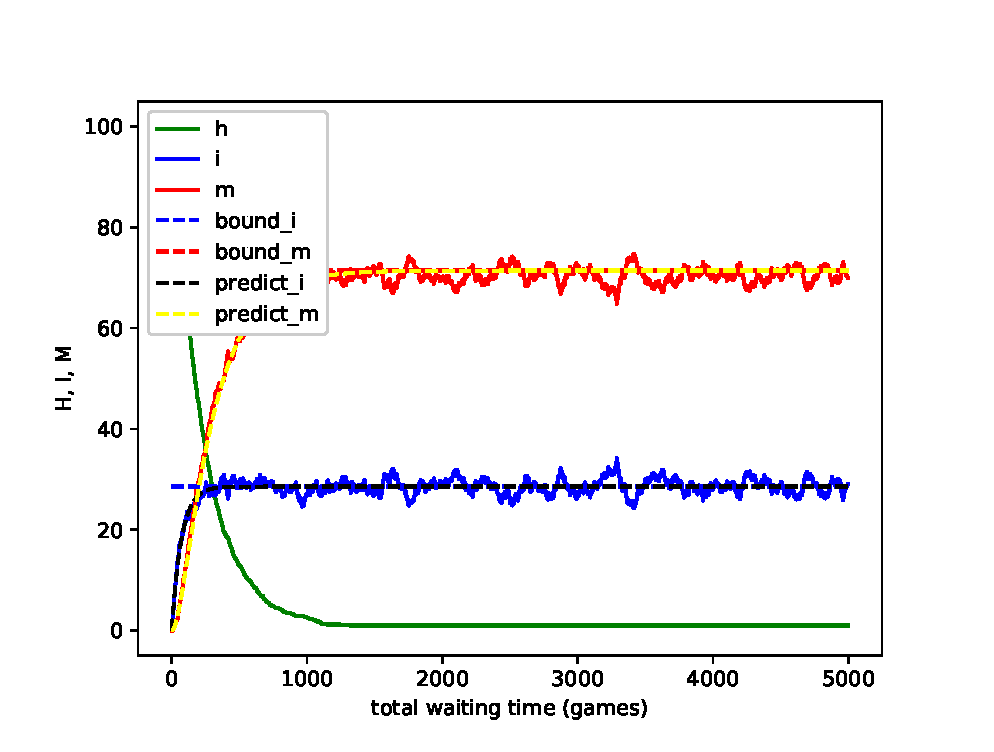
\includegraphics[width=.45\textwidth]{fig/twohop_predict_sim.eps}
  \caption{$I(t)$ and $M(t)$ with time $t$ obtained from prediction and simulations
  when $\beta = 0.004$, $\rho = 0.01$ and $N=100$. Here $h$ and $i$ is the mean value of $20$ simulations.}
  \label{fig:twohop_predict_wod}
\end{figure}
We can find that when $t \rightarrow + \infty$, $I(t) \rightarrow \frac{ \beta N }{ \beta + \rho }$
and $M(t) \rightarrow \frac{ \rho N }{ \beta + \rho }$.

\subsection{Object Function}
The expected number of nodes, which declare that holding the messages, in the range $t \in (0, T]$
can be viewed as the contribution of the relay nodes,
which will be proportional to the reward paid from the message sender.
Thus the total paid reward for the selfish behaviors is
\begin{small}
\begin{equation}
\nonumber
\begin{aligned}
J &= \int_{0}^{T} M(t) dt,
\end{aligned}
\end{equation}
\end{small}
where $T$ is the Time to Live (TTL) of message $m$.
$M(t)$ is the waste of the reward at the instant time $t$.
which also can be calculated.
Based on the calculated result,
We can find that $()\%$ reward are paid to the nodes without messages.

